\documentclass{article}
\usepackage[utf8]{inputenc}
\usepackage{tikz}

\usepackage{xcolor}

\title{vfi-gridworld}
\author{tarikocaktan}
\date{May 2021}

\begin{document}

\maketitle


%%% Starting gridworld
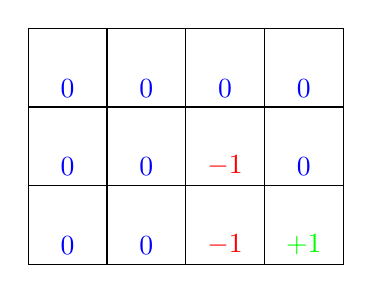
\begin{tikzpicture}

% First row of boxes
\draw (0,0) -- (0.5,0) node[above] { {\color{blue} $0$} } -- (1,0) -- (1,1) -- (0,1) -- (0,0) ;
\draw (1,0) -- (1.5,0) node[above] { {\color{blue} $0$} } -- (2,0) -- (2,1) -- (1,1) -- (1,0);
\draw (2,0) -- (2.5,0) node[above] { {\color{red} $-1$} } -- (3,0) -- (3,1) -- (2,1) -- (2,0);
\draw (3,0) -- (3.5,0) node[above] { {\color{green} $+1$} } -- (4,0) -- (4,1) -- (3,1) -- (3,0);


% Second row of boxes
\draw (0,1) -- (0.5,1) node[above] { {\color{blue} $0$} } -- (1,1) -- (1,2) -- (0,2) -- (0,1);
\draw (1,1) -- (1.5,1) node[above] { {\color{blue} $0$} } -- (2,1) -- (2,2) -- (1,2) -- (1,1);
\draw (2,1) -- (2.5,1) node[above] { {\color{red} $-1$} } -- (3,1) -- (3,2) -- (2,2) -- (2,1);
\draw (3,1) -- (3.5,1) node[above] { {\color{blue} $0$} } -- (4,1) -- (4,2) -- (3,2) -- (3,1);

% Third row of boxes
\draw (0,2) -- (0.5,2) node[above] { {\color{blue} $0$} } -- (1,2) -- (1,3) -- (0,3) -- (0,2);
\draw (1,2) -- (1.5,2) node[above] { {\color{blue} $0$} } -- (2,2) -- (2,3) -- (1,3) -- (1,2);
\draw (2,2) -- (2.5,2) node[above] { {\color{blue} $0$} } -- (3,2) -- (3,3) -- (2,3) -- (2,2);
\draw (3,2) -- (3.5,2) node[above] { {\color{blue} $0$} } -- (4,2) -- (4,3) -- (3,3) -- (3,2);


\end{tikzpicture}


\hspace{15cm}


%%% Gridworld after solution
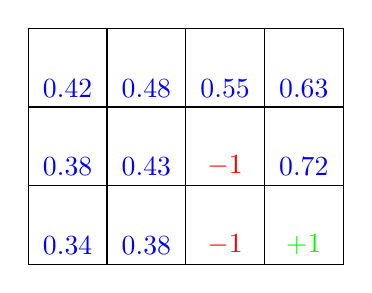
\begin{tikzpicture}

% First row of boxes
\draw (0,0) -- (0.5,0) node[above] { {\color{blue} $0.34$} } -- (1,0) -- (1,1) -- (0,1) -- (0,0) ;
\draw (1,0) -- (1.5,0) node[above] { {\color{blue} $0.38$} } -- (2,0) -- (2,1) -- (1,1) -- (1,0);
\draw (2,0) -- (2.5,0) node[above] { {\color{red} $-1$} } -- (3,0) -- (3,1) -- (2,1) -- (2,0);
\draw (3,0) -- (3.5,0) node[above] { {\color{green} $+1$} } -- (4,0) -- (4,1) -- (3,1) -- (3,0);


% Second row of boxes
\draw (0,1) -- (0.5,1) node[above] { {\color{blue} $0.38$} } -- (1,1) -- (1,2) -- (0,2) -- (0,1);
\draw (1,1) -- (1.5,1) node[above] { {\color{blue} $0.43$} } -- (2,1) -- (2,2) -- (1,2) -- (1,1);
\draw (2,1) -- (2.5,1) node[above] { {\color{red} $-1$} } -- (3,1) -- (3,2) -- (2,2) -- (2,1);
\draw (3,1) -- (3.5,1) node[above] { {\color{blue} $0.72$} } -- (4,1) -- (4,2) -- (3,2) -- (3,1);

% Third row of boxes
\draw (0,2) -- (0.5,2) node[above] { {\color{blue} $0.42$} } -- (1,2) -- (1,3) -- (0,3) -- (0,2);
\draw (1,2) -- (1.5,2) node[above] { {\color{blue} $0.48$} } -- (2,2) -- (2,3) -- (1,3) -- (1,2);
\draw (2,2) -- (2.5,2) node[above] { {\color{blue} $0.55$} } -- (3,2) -- (3,3) -- (2,3) -- (2,2);
\draw (3,2) -- (3.5,2) node[above] { {\color{blue} $0.63$} } -- (4,2) -- (4,3) -- (3,3) -- (3,2);


\end{tikzpicture}



\hspace{15cm}


%%% Gridworld after solution
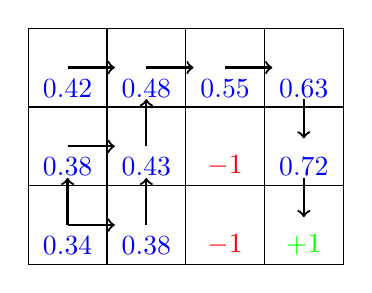
\begin{tikzpicture}

% First row of boxes
\draw (0,0) -- (0.5,0) node[above] { {\color{blue} $0.34$} } -- (1,0) -- (1,1) -- (0,1) -- (0,0) ;
\draw (1,0) -- (1.5,0) node[above] { {\color{blue} $0.38$} } -- (2,0) -- (2,1) -- (1,1) -- (1,0);
\draw (2,0) -- (2.5,0) node[above] { {\color{red} $-1$} } -- (3,0) -- (3,1) -- (2,1) -- (2,0);
\draw (3,0) -- (3.5,0) node[above] { {\color{green} $+1$} } -- (4,0) -- (4,1) -- (3,1) -- (3,0);
% Cell (0,0)
\draw[thick,->] (0.5,0.5) -- (1.1,0.5);
\draw[thick,->] (0.5,0.5) -- (0.5,1.1);
% Cell (1,0)
\draw[thick,->] (1.5,0.5) -- (1.5,1.1);

% Second row of boxes
\draw (0,1) -- (0.5,1) node[above] { {\color{blue} $0.38$} } -- (1,1) -- (1,2) -- (0,2) -- (0,1);
\draw (1,1) -- (1.5,1) node[above] { {\color{blue} $0.43$} } -- (2,1) -- (2,2) -- (1,2) -- (1,1);
\draw (2,1) -- (2.5,1) node[above] { {\color{red} $-1$} } -- (3,1) -- (3,2) -- (2,2) -- (2,1);
\draw (3,1) -- (3.5,1) node[above] { {\color{blue} $0.72$} } -- (4,1) -- (4,2) -- (3,2) -- (3,1);
% Cell (0,1)
\draw[thick,->] (0.5,1.5) -- (1.1,1.5);
%\draw[thick,->] (0.5,1.5) -- (0.5,2.1);
% Cell (1,1)
\draw[thick,->] (1.5,1.5) -- (1.5,2.1);

% Third row of boxes
\draw (0,2) -- (0.5,2) node[above] { {\color{blue} $0.42$} } -- (1,2) -- (1,3) -- (0,3) -- (0,2);
\draw (1,2) -- (1.5,2) node[above] { {\color{blue} $0.48$} } -- (2,2) -- (2,3) -- (1,3) -- (1,2);
\draw (2,2) -- (2.5,2) node[above] { {\color{blue} $0.55$} } -- (3,2) -- (3,3) -- (2,3) -- (2,2);
\draw (3,2) -- (3.5,2) node[above] { {\color{blue} $0.63$} } -- (4,2) -- (4,3) -- (3,3) -- (3,2);
% Cell (0,2)
\draw[thick,->] (0.5,2.5) -- (1.1,2.5);
% Cell (1,2)
\draw[thick,->] (1.5,2.5) -- (2.1,2.5);
% Cell ()
\draw[thick,->] (2.5,2.5) -- (3.1,2.5);
% Cell ()
\draw[thick,->] (3.5,2.1) -- (3.5,1.6);
% Cell ()
\draw[thick,->] (3.5,1.1) -- (3.5,0.6);

\end{tikzpicture}





\end{document}
